% ============================================
%       Presentation Compile Setting
% ============================================

\documentclass[8pt, aspectratio=169]{beamer} % for full presentation
% \documentclass[8pt, aspectratio=169, handout]{beamer} % without animation and notes
% \documentclass[8pt, aspectratio=169, handout, draft]{beamer} % for draft mode
% \documentclass[8pt, aspectratio=169, handout]{beamer} \setbeameroption{show only notes} % for notes only

% ============================================
%           MIC Lab template
% ============================================
\newcommand{\template}{../template}

% \input{\template/macros/macros_general.tex}
% \input{\template/macros/macros_math.tex}
% \input{\template/symbols/symbols_NN.tex}
% \input{\template/symbols/symbols_robot.tex}
% Add more macros/symbols as needed

\newcommand{\logoOne}{\template/figs/logo_KAIST_simple.png}
\newcommand{\logoTwo}{\template/figs/logo_MIC.png}
\newcommand{\logoTopRight}{\template/figs/logo_MIC_white.png}

% ============================================
%           Flux Theme
% ============================================

% Use roboto Font (recommended)
% \usepackage[sfdefault]{roboto}
\usepackage[utf8]{inputenc}
\usepackage[T1]{fontenc}

% Define where theme files are located. ('/styles')
\usepackage{styles/fluxmacros}
\usefolder{styles}
% Use Flux theme v0.1 beta
% Available style: asphalt, blue, red, green, gray, dding (custom)
\usetheme[style=dding]{flux}

% ============================================
%         Additional Packages
% ============================================

\usepackage{booktabs}
\usepackage{colortbl}
\usepackage{ragged2e}
\usepackage{schemabloc}
\usepackage{multirow}
\usepackage{multicol}
\usepackage{kotex}
\usepackage{media9}
\usepackage{pgfpages}
% \setbeameroption{show notes} % Show notes separately
% \setbeameroption{show notes on second screen=right} % Show notes on the presenter screen

% ============================================
%         Colors and Macros
% ============================================

% https://latexcolor.com % colo r list 
\definecolor{airforceblue}{rgb}{0.36, 0.54, 0.66}
\definecolor{awesome}{rgb}{1.0, 0.13, 0.32}
\newcommand{\ctxt}[2]{{\color{#1}{#2}\color{black}}}
\newcommand{\cred}[1]{{\ctxt{awesome}{#1}}}
\newcommand{\cblue}[1]{{\ctxt{airforceblue}{#1}}}

% ============================================
%         Title Page
% ============================================
\title{
    Constrained Reinforcement Learning
} 
\subtitle{
    \textit{2025 MIC Symposium}\\
}
\author{
  \textbf{\cblue{Minseok Seo}}\inst{1},  % Emphasize the presenter!
}
\date{{September 5, 2025}}
\institute{%
    \begin{minipage}[c]{\linewidth}
      \centering
      \inst{1}%
      Mobility Intelligence and Control Laboratory (MIC Lab) \\
      CCS Graduate School of Mobility \\
      Korea Advanced Institute of Science and Technology (KAIST)
  \end{minipage}
}
\setbeamerfont{institute}{size=\normalsize}

\titlegraphic{\logoTopRight}


%~~~~~~~~~~~~~~~~~~~~~~~~~~~~~~~~~~~~~~~~~~~~~~~~~~~~~~~~~~~~~~~~~~~~~~~~~~~~~~
\AtBeginSection[]{%
  \frame<beamer>{ 
    \frametitle{Outline}   
    \tableofcontents[currentsection] 
  }
}

% Use the following code to show section and subsection titles at the beginning of each section and subsection
% \AtBeginSubsection[]{%
%   \begin{frame}
%   \vfill
%   \centering
%     \insertsectionhead
%     \\
%     \large\textbf{\insertsubsectionhead}
%   \vfill
%   \end{frame}
% }
%~~~~~~~~~~~~~~~~~~~~~~~~~~~~~~~~~~~~~~~~~~~~~~~~~~~~~~~~~~~~~~~~~~~~~~~~~~~~~~


\begin{document}

%~~~~~~~~~~~~~~~~~~~~~~~~~~~~~~~~~~~~~~~~~~~~~~~~~~~~~~~~~~~~~~~~~~~~~~~~~~~~~~
\titlepage 


\begin{frame}{Outline}
  \tableofcontents
\end{frame}

\note[enumerate]
{
  \item Hello everyone, I am Minseok.
  \item I'm currently working as a part-time researcher.
  \item Today, I would like to briefly introduce the research I have been working on.
  \item Before I begin, please understand if I say something strange, because I'm not goot at speaking in English.
  \item So, let's get started.
  \item The order of my presentation is as follows.
}

%~~~~~~~~~~~~~~~~~~~~~~~~~~~~~~~~~~~~~~~~~~~~~~~~~~~~~~~~~~~~~~~~~~~~~~~~~~~~~~

% ============================================
%         Introduction
% ============================================

\section{Introduction}

%~~~~~~~~~~~~~~~~~~~~~~~~~~~~~~~~~~~~~~~~~~~~~~~~~~~~~~~~~~~~~~~~~~~~~~~~~~~~~~

\subsection{Motivation}


\note[enumerate]
{
  \item First, the introduction.
}

\begin{frame}{\insertsubsectionhead}{Autonomous Driving}


  \vspace{0.5cm}

  {
    \begin{figure}
      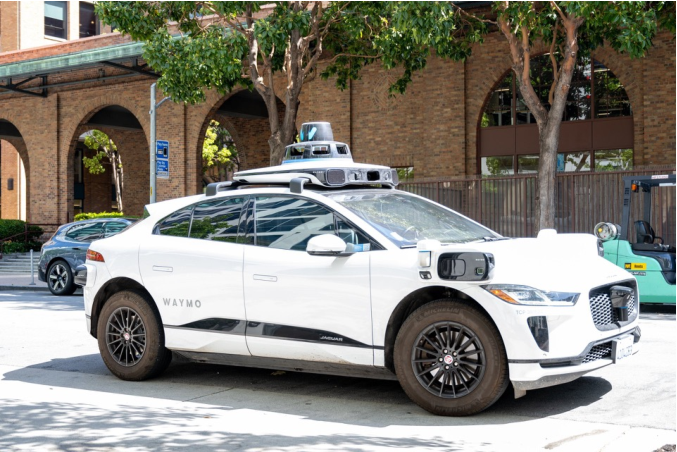
\includegraphics[width=0.45\textwidth]{figures/waymo.pdf}
      \hspace{1cm}
      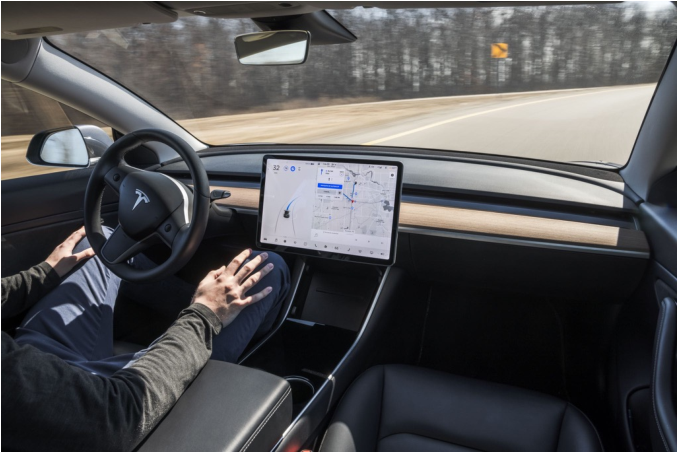
\includegraphics[width=0.45\textwidth]{figures/tesla.pdf}
      \caption{Waymo and Tesla}
    \end{figure}
  }

\end{frame}

\note[enumerate]
{
  \item When I was young, I really liked cars and was very interested in self-driving technology.
  \item Currently, I think the most well-known companies in autonomous driving are Waymo and Tesla.
  \item Since more information is available about Tesla, I will focus on Tesla in my presentation.
}

\begin{frame}{\insertsubsectionhead}{Supervised Learning}

  \vspace{0.5cm}

  {
    \begin{figure}
      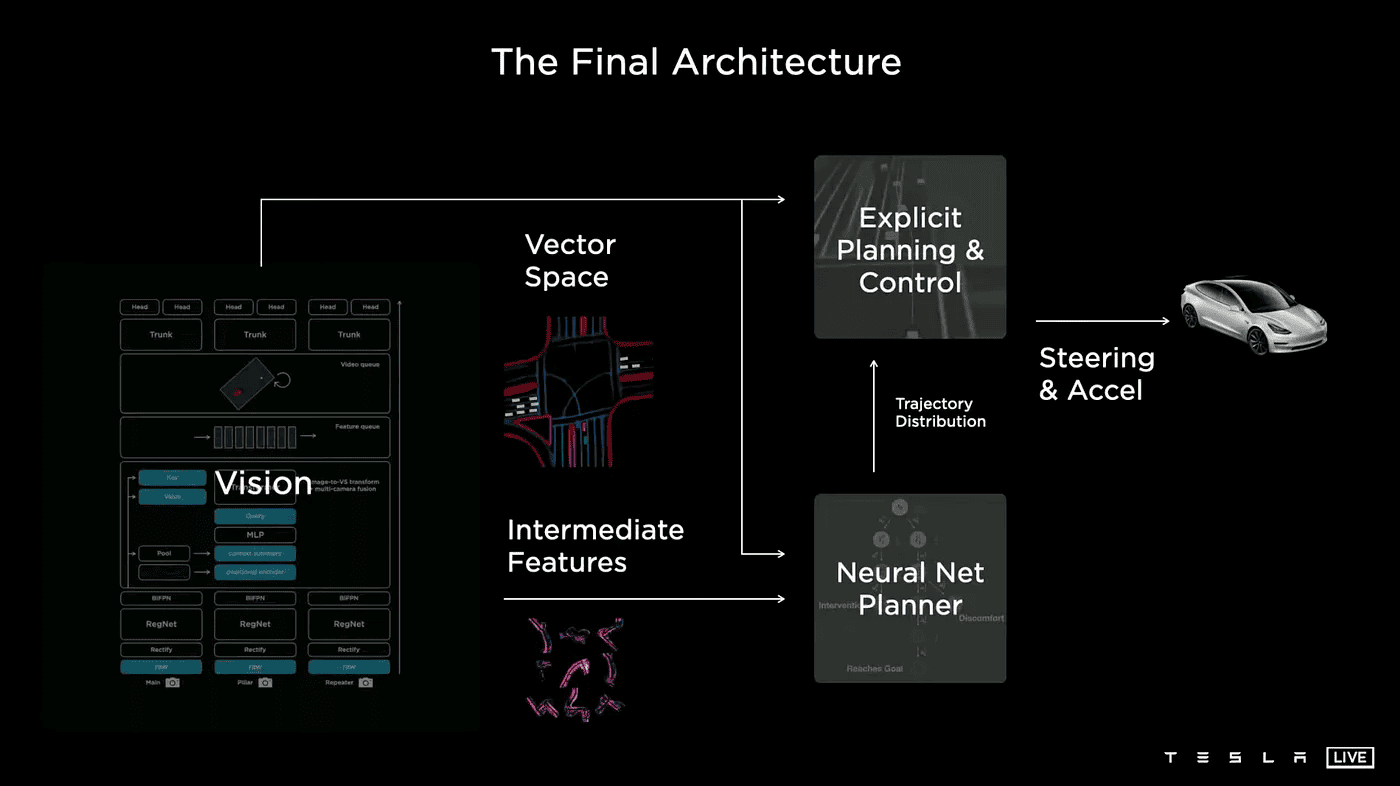
\includegraphics[width=0.7\textwidth]{figures/tesla-architecture.png}
      \caption{Tesla's Architecture in 2021 (source: \href{https://www.youtube.com/live/j0z4FweCy4M?si=vEB4egdqDOVpmpLu}{AI Day 2021})}
    \end{figure}
  }
\end{frame}

\note[enumerate]
{
  \item Tesla pursues an approach where data from cameras is processed by a neural network, and then used to generate the appropriate control inputs in an end-to-end manner.
  \item To achieve this, they use a large amount of human-labeled data to train the neural network.
}

\begin{frame}{\insertsubsectionhead}{Supervised Learning}

  {
    \begin{figure}
      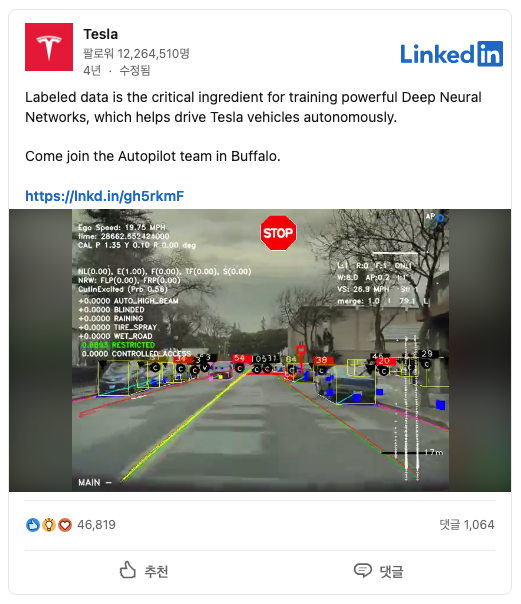
\includegraphics[width=0.25\textwidth]{figures/tesla-label.png}
      \caption{Tesla’s recruitment post for data labeling positions}
    \end{figure}

    \onslide <1->
    {
      \begin{itemize}
        \item <2-> Supervised learning requires \textcolor{red}{a large amount of labeled data.}
        \item <3-> Since it is created by humans, it is \textcolor{red}{expensive.}
        \item <4-> The performance of supervised learning is \textcolor{red}{depends on human-labeled data.}
      \end{itemize}
    }
  }

\end{frame}

\note[enumerate]
{
  \item To support this, about four years ago, Tesla posted job openings on LinkedIn for data labeling.
  \item Supervised learning is effective, but it requires a large amount of data.
  \item Since the labels are made by humans, it is also very costly, and the performance of supervised learning depends on human-labeled data.
  \item Therefore, it is difficult for academic labs like ours to use this approach.
}
%~~~~~~~~~~~~~~~~~~~~~~~~~~~~~~~~~~~~~~~~~~~~~~~~~~~~~~~~~~~~~~~~~~~~~~~~~~~~~~

\subsection{Reinforcement Learning (RL)}

\begin{frame}{\insertsubsectionhead}

  \centering
  \begin{columns}[T,totalwidth=\textwidth]
    % Alphago
    \column{0.32\textwidth}
      \centering
      \textbf{Alpha Go} \cite{silver2016mastering}
      
\includegraphics[width=\linewidth,height=0.5625\linewidth]{figures/alphago.jpg}

    % DQN
    \column{0.32\textwidth}
      \centering
      \textbf{Deep Q-Network} \cite{mnih2013playing}
      \includemedia[
        width=\linewidth,
        height=0.5625\linewidth,
        activate=pageopen,
        addresource=figures/dqn.mp4,
        flashvars={source=figures/dqn.mp4&autoPlay=true&loop=true}
      ]{}{VPlayer.swf}

    % Walker
    \column{0.32\textwidth}
      \centering
      \textbf{Proximal Policy Optimization} \cite{schulman2017proximal}
      \includemedia[
        width=\linewidth,
        height=0.5625\linewidth,
        activate=pageopen,
        addresource=figures/walker.mp4,
        flashvars={source=figures/walker.mp4&autoPlay=true&loop=true}
      ]{}{VPlayer.swf}
  \end{columns}

\end{frame}

\note[enumerate]
{
  \item Because of these reasons, and with the progress of reinforcement learning, many studies are now trying to apply reinforcement learning to various real-world problems.
  \item I am also conducing research on reinforcement learning.
}

\begin{frame}{\insertsubsectionhead}

  \begin{figure}
    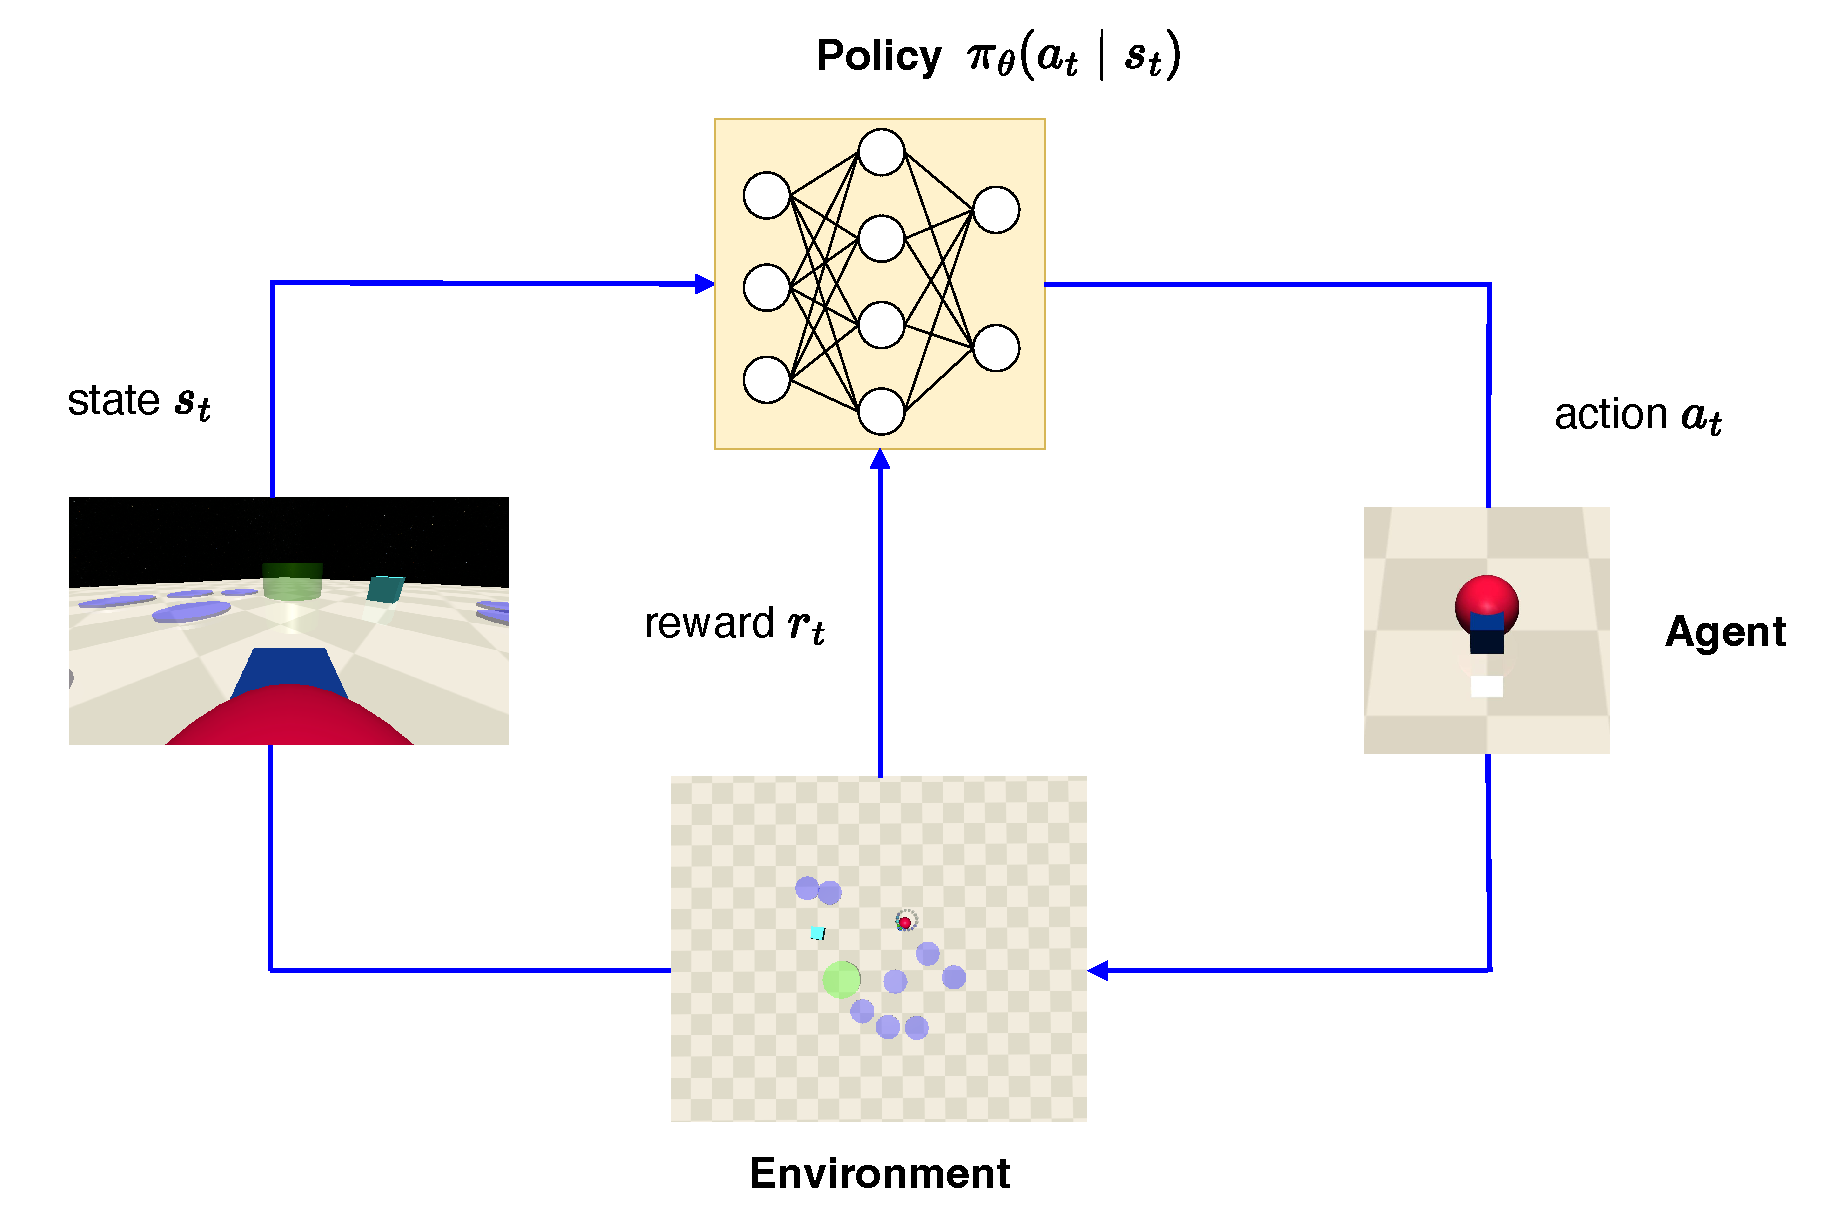
\includegraphics[width=0.6\textwidth]{figures/rl1.pdf}
    \caption{Overview of the reinforcement learning framework}
  \end{figure}

\end{frame}

\note[enumerate]
{
  \item This is an overview of the reinforcement learning framework.
  \item The agent observes the current state from the environment and based on this state, the policy decides an action.
  \item Then, agent takes this action, and as a result, the agent receives a reward from the environment.
  \item By repeating this process, agent learns a policy that maximizes the cumulative reward.
}


\begin{frame}{\insertsubsectionhead}

  \begin{figure}
    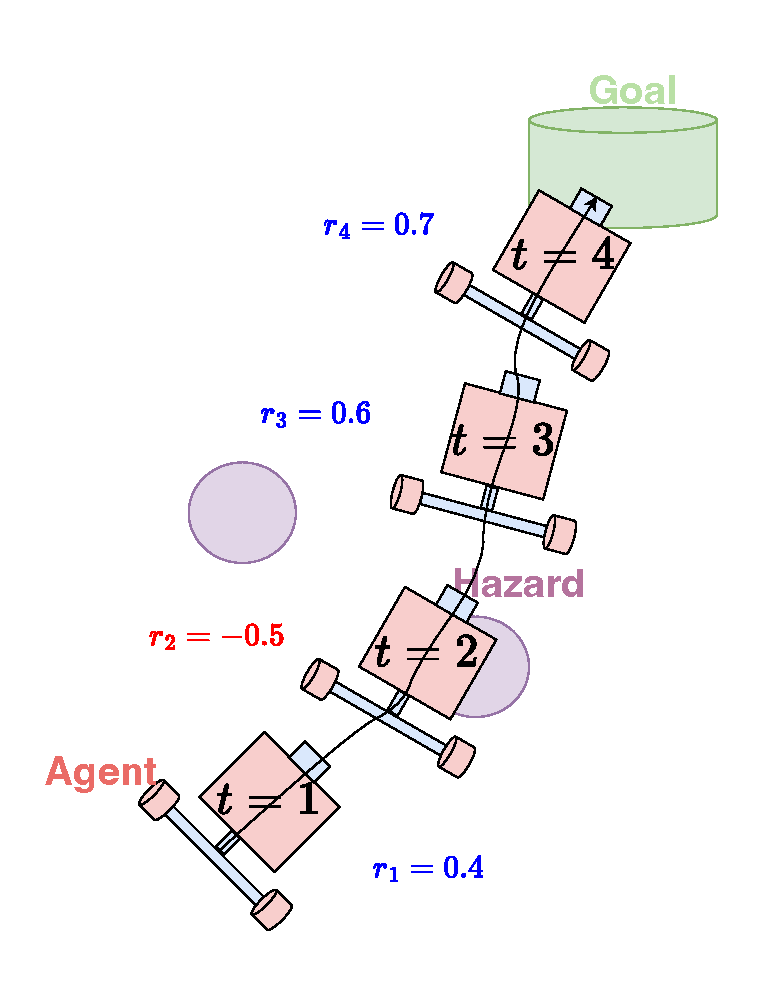
\includegraphics[width=0.3\textwidth]{figures/rl2.pdf}
    \caption{Illustration of sequential decision making: the agent receives a reward after each action.}
  \end{figure}

\end{frame}

\note[enumerate]
{
  \item This illustration describes the process over time.
  \item At each time step, the agent takes an action and receives a reward.
  \item In this example, we want to learn a policy to avoid obstacles, so stepping on an obstacle is defined to give a negative reward.
  \item Agent receives a positive reward as it approaches the goal.
}


\begin{frame}{\insertsubsectionhead}{Objective of RL}
  \begin{itemize}
    \item Policy parameterized by $\theta$, denoted as $\pi_\theta(a|s)$
    \item Goal: find the optimal policy $\pi^*_\theta$ that maximizes the expected cumulative reward
  \end{itemize}

  \begin{equation}
    \begin{aligned}
      \theta^* &= \arg\max_\theta J(\theta) \\
      J(\theta) &= \mathbb{E}_{\tau \sim \pi_\theta} \left[\sum^T_{t = 0} r_t \right]
    \end{aligned}
  \end{equation}

\end{frame}

\note[enumerate]
{
  \item If we represent this process with equations, it can be written as follows.
  \item First, we assume that the policy is parameterized by theta.
  \item Our goal is to find a policy pi with parameters theta that maximizes the cumulative reward.
}


\begin{frame}{\insertsubsectionhead}{Challenges of RL}

  \begin{enumerate}
    \item<2-> \textcolor{red}{Reward engineering} can induce desired behaviors (multi-objective), but it is time-consuming and difficult
    \item<3-> Even with reward engineering, the agent may still take \textcolor{red}{unsafe actions}
      \begin{itemize}
        \item<3-> Reward hacking  \cite{weng2024rewardhack}
        \item <3-> Out-of-distribution cases (unseen during training)
      \end{itemize}
  \end{enumerate}

  \uncover<4->{
    \begin{block}{My research}
      Challenges 2 \& 3: learning safe policies without relying on reward engineering
    \end{block}
  }
\end{frame}

\note[enumerate]
{
  \item However, reinforcement learning also faces several challenges.
  \item Among them, I will focus on two challenges.
  \item First, to make the agent learn the desired behavior, reward engineering is required.
  \item However, it is very difficult and time-consuming.
  \item Even if the agent has learned the desired behaviors well through reward engineering, it may still take unsafe actions.
  \item This can happen due to reward hacking or because the agent encounters situations that it has never seen during training, that is, out-of-distribution cases.
  \item Therefore, my research aims to learn a safe policy without relying on reward engineering.
}

% ============================================
%         Constrained RL Page
% ============================================

\section{Constrained Reinforcement Learning}

%~~~~~~~~~~~~~~~~~~~~~~~~~~~~~~~~~~~~~~~~~~~~~~~~~~~~~~~~~~~~~~~~~~~~~~~~~~~~~~

\subsection{Constrained Reinforcement Learning (Constrained RL)}

\note[enumerate]
{
  \item In the next section I will introduce constrained reinforcement learning, which is one of the methodologies to address these challenges.
}

\begin{frame}{\insertsubsectionhead}
  \begin{figure}
    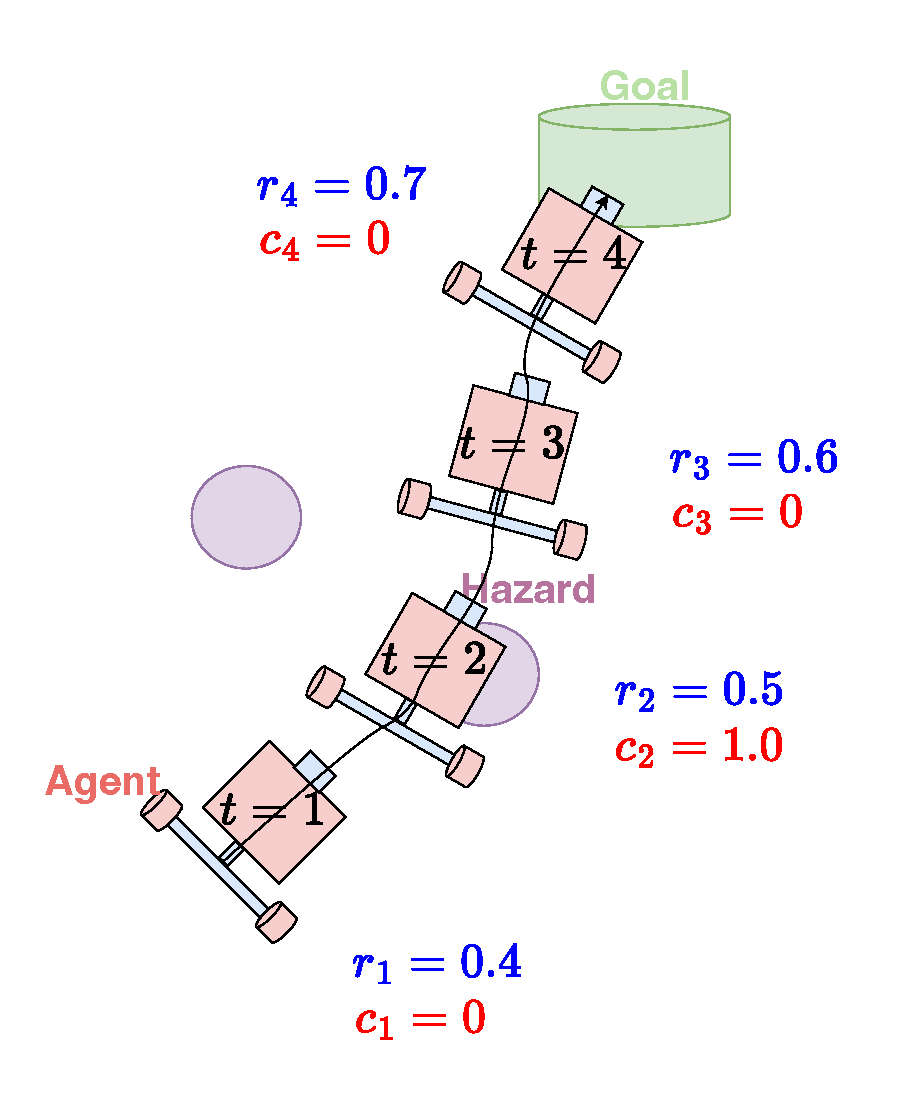
\includegraphics[width=0.35\textwidth]{figures/constrained-rl1.pdf}
    \caption{Constrained RL example — agent trajectory with rewards (blue) and costs (red)}
  \end{figure}
\end{frame}

\note[enumerate]
{
  \item Unlike what we saw earlier in standard RL, constrained RL introduces an additional cost function.
  \item Rewards encourage the desired behavior, while the cost function is used to discourage the undesired ones.
}
%~~~~~~~~~~~~~~~~~~~~~~~~~~~~~~~~~~~~~~~~~~~~~~~~~~~~~~~~~~~~~~~~~~~~~~~~~~~~~~

\subsection{Constrained Policy Optimization Problem}

\begin{frame}{\insertsubsectionhead}

  \begin{equation}
    \begin{aligned}
      \theta^* &= \arg\max_\theta J(\theta) \\
      J(\theta) &= \mathbb{E}_{\tau \sim \pi_\theta} \left[ \sum^T_{t = 0} r_t \right] \; \text{subject to} \; \mathbb{E}_{\tau \sim \pi_\theta} \left[ \sum^T_{t = 0} c_t \right] \leq d
    \end{aligned}
  \end{equation}

  \vspace{0.5cm}

  \begin{itemize}
    \item <2-> Find a policy that maximizes rewards while satisfying constraints.
    \item <3-> Directly solving \textcolor{red}{constrained optimization} is difficult.
    \item <4-> By applying Lagrangian relaxation, we can convert it to an \textcolor{blue}{unconstrained problem.}
  \end{itemize}

\end{frame}

\note[enumerate]
{
  \item If we express this in equations, it looks like this.
  \item At each step, the agent receives both a reward and a cost.
  \item The goal is to find a policy that maximizes the cumulative reward, while keeping the cumulative cost below a threshold d.
  \item In other words, the value of the cumulative cost becomes the constraint. 
  \item However, solving this problem directly is difficult.
  \item There are several approaches to solve this problem, but here I will only explain the method of transforming it into an unconstrained problem using Lagrangian relaxation.
}


\begin{frame}{\insertsubsectionhead}

  \begin{equation}
    \begin{aligned}
      \theta^* &= \arg\max_\theta \mathcal{L}(\theta, \lambda) \\
      \mathcal{L}(\theta, \lambda) &= \mathbb{E}_{\tau \sim \pi_\theta} \left[ \sum^T_{t = 0} r_t \right] - \lambda \left( \mathbb{E}_{\tau \sim \pi_\theta} \left[ \sum^T_{t = 0} c_t \right] - d \right)
    \end{aligned}
  \end{equation}

  \vspace{0.5cm}

  \begin{equation}
    \lambda \leftarrow \left[ \lambda + \beta\left( \hat{J}_c - d \right) \right]_+
  \end{equation}

  \vspace{0.5cm}

  Penalty ($\lambda$) increases when constraints are violated → policy is encouraged to satisfy them.

  % Whenever the agent violates the constraints, the penalty (Lagrange multiplier, $\lambda$) is increased, thereby encouraging the policy to satisfy the constraints.

\end{frame}

\note[enumerate]
{
  \item The transformed equation is as follows.
  \item The Lagrange multiplier is a scalar, and it is increased when the constraint is violated and decreased when the constraint is satisfied.
  \item In this way, it encourages the policy to satisfy the constraints.
}

\begin{frame}{\insertsubsectionhead}
  \begin{figure}
    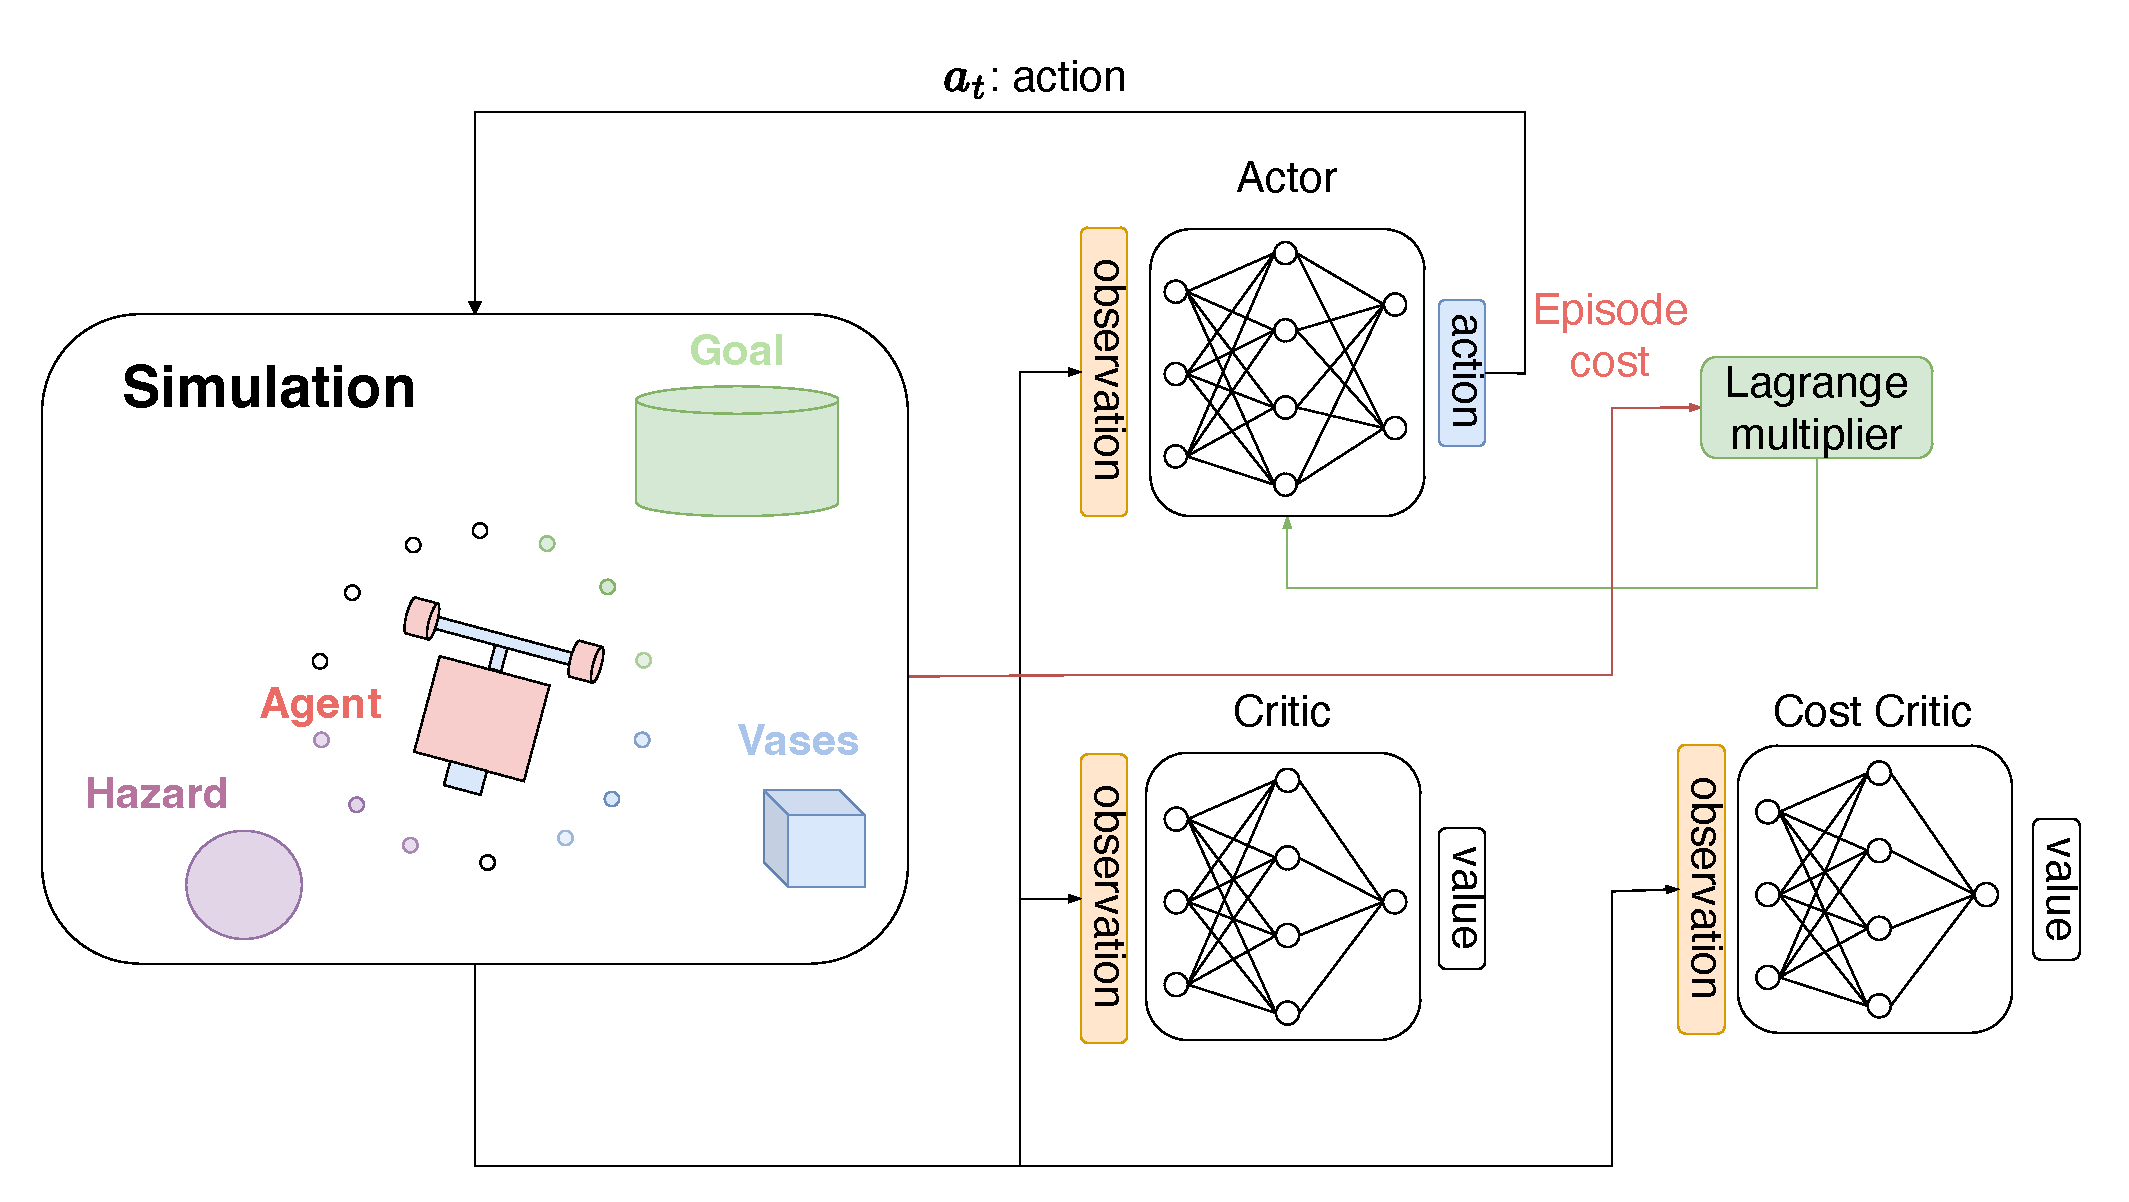
\includegraphics[width=0.6\textwidth]{figures/ppo-lag.pdf}
    \caption{Overview of the Constrained RL with Lagrangian relaxation}
  \end{figure}
\end{frame}

\begin{frame}{\insertsubsectionhead}

  In Constrained RL, constraints are imposed on the trajectory level.

  \begin{figure}
    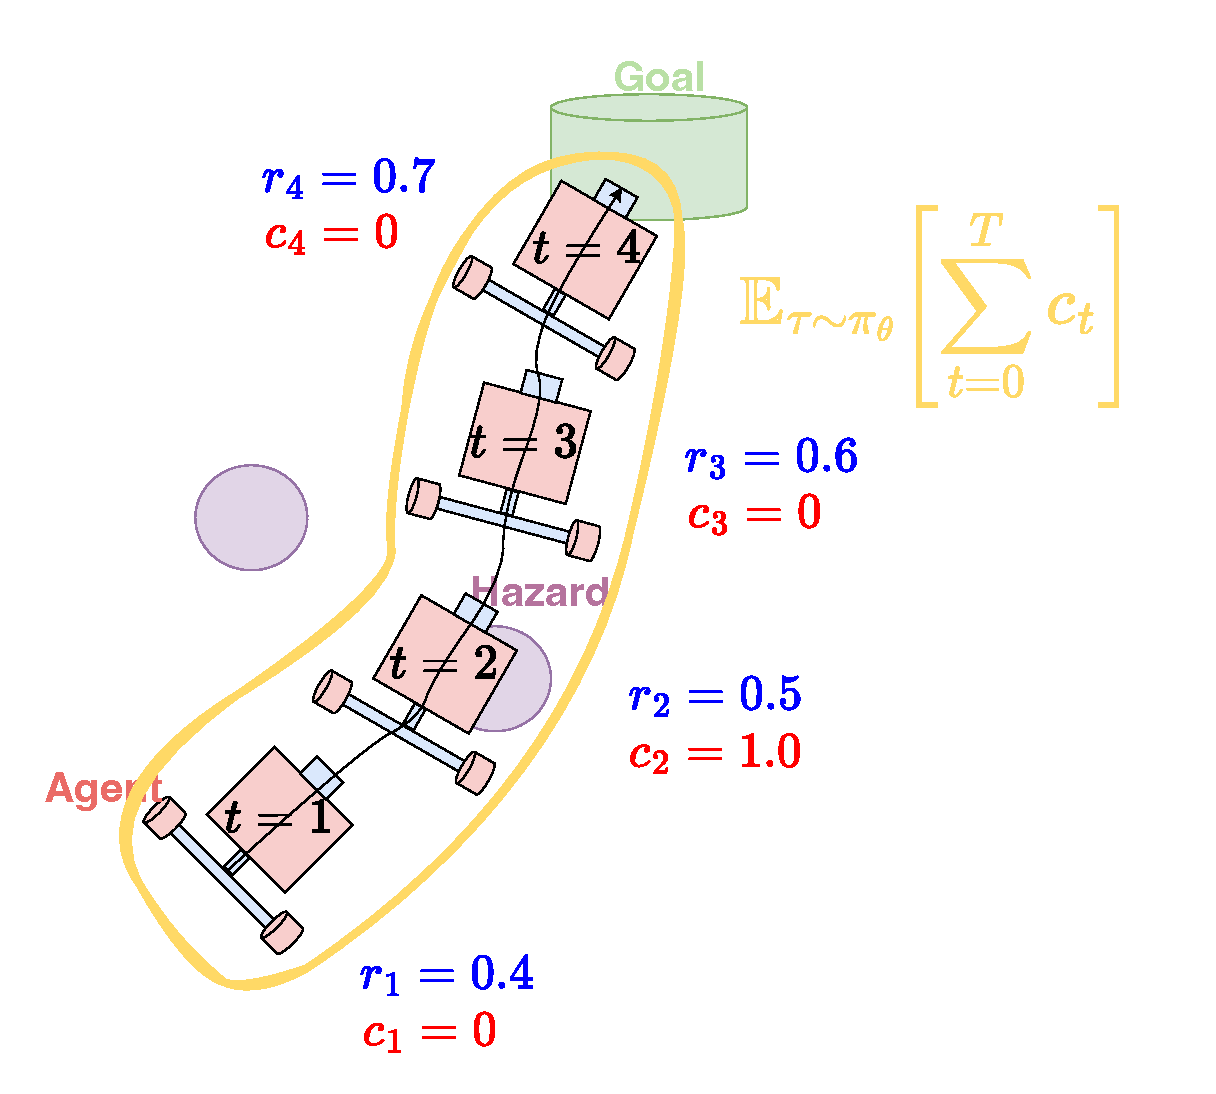
\includegraphics[width=0.3\textwidth]{figures/constrained-rl2.pdf}
    \caption{Constrained RL example — agent trajectory with rewards (blue) and costs (red)}
  \end{figure}

  \uncover<2->{\textbf{Wouldn’t imposing constraints at the state level allow for more precise constraint enforcement?}}

\end{frame}

\note[enumerate]
{
  \item Earlier, I metioned that the constraint is defined so that the total cost accumulated until the end of an episode does not exceed threshold.
  \item As shown in the figure, this corresponds to imposing the constraint at the trajectory level.
  \item However, since there are many uncertainties from beginning to the end of an episode, one may wonder if it would be better to impose the constraint at each state, step by step, rather than only at the trajectory level.
}

%~~~~~~~~~~~~~~~~~~~~~~~~~~~~~~~~~~~~~~~~~~~~~~~~~~~~~~~~~~~~~~~~~~~~~~~~~~~~~~

\subsection{State-wise Constrained Policy Optimization}

\begin{frame}{\insertsubsectionhead}

  In state-wise constrained MDPs, constraints are imposed on each state.

  \begin{figure}
    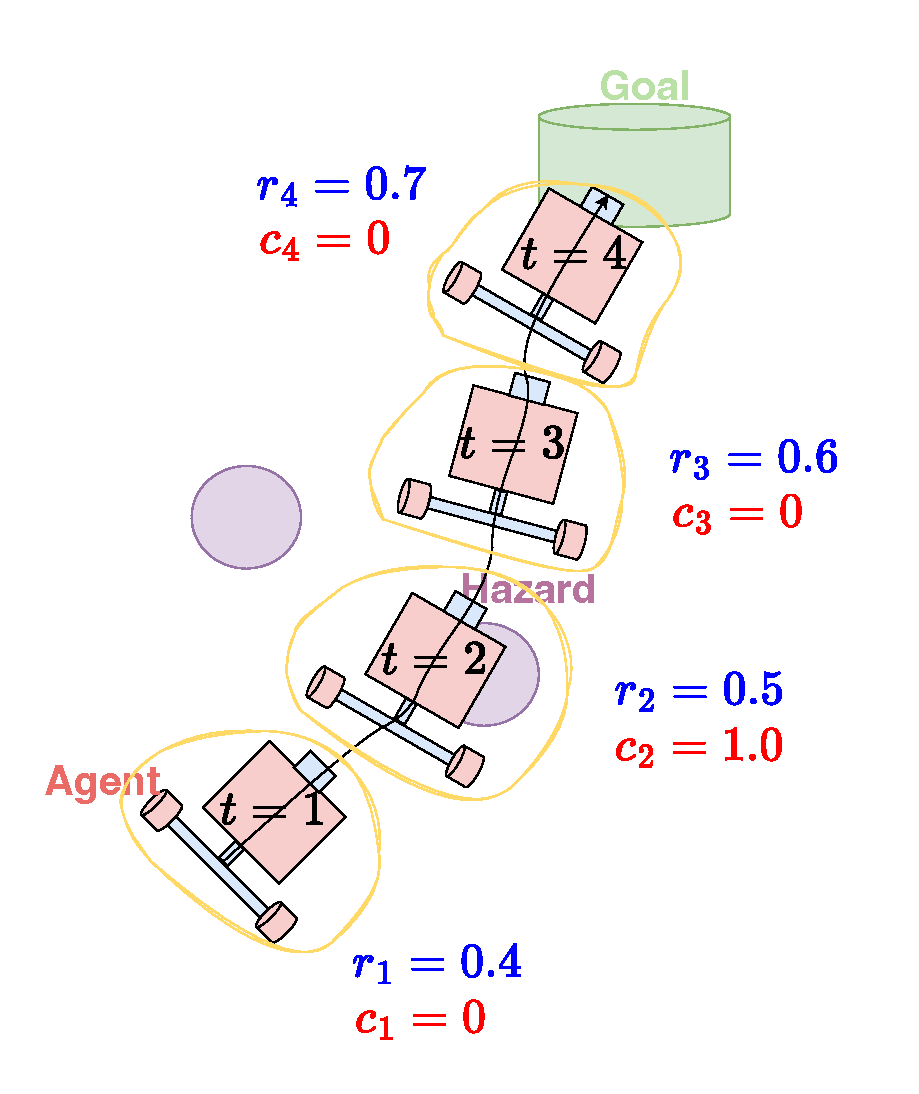
\includegraphics[width=0.25\textwidth]{figures/statewise-constrained-rl.pdf}
    \caption{State-wise constrained RL example — agent trajectory with rewards (blue) and costs (red)}
  \end{figure}

\end{frame}

\note[enumerate]
{
  \item This was actually the topic of my master's thesis.
  \item In fact, this idea was suggested by professor.
  \item Previously, the constraint was defined at the trajectory level, but now it is defined at each state.
}

\begin{frame}{\insertsubsectionhead}{Proposed Method}

  \begin{equation}
    \begin{aligned}
      \pi^* &= \arg\max_{\pi_\theta} J(\theta) \\
      J(\theta) &= \mathbb{E}_{\tau \sim \pi_\theta} \left[ \sum^T_{t = 0} r_t \right] \; \text{subject to} \; \mathbb{E}_{\tau \sim \pi_\theta}  [c(s, a)] \leq w, \quad \forall s \in S
    \end{aligned}
  \end{equation}

  \begin{equation}
    \lambda(s) \leftarrow \lambda(s) + \beta(\hat{J}_c - w)
  \end{equation}

  \vspace{0.5cm}

  \uncover<2->{\textbf{The Lagrange multiplier is replaced by a neural network's output instead of a scalar.}}

\end{frame}

\note[enumerate]
{
  \item If we express this in equation, it looks like this.
  \item Previously, the Lagrange multiplier was a scalar, but now it becomes a network, so that different multipliers are used for different states.
  \item As I mentioned before, the network is updated so that the multiplier decreases when the constraint is satisfied, and increases when it is not.
}

\begin{frame}{\insertsubsectionhead}{Proposed Method}

  \begin{figure}
    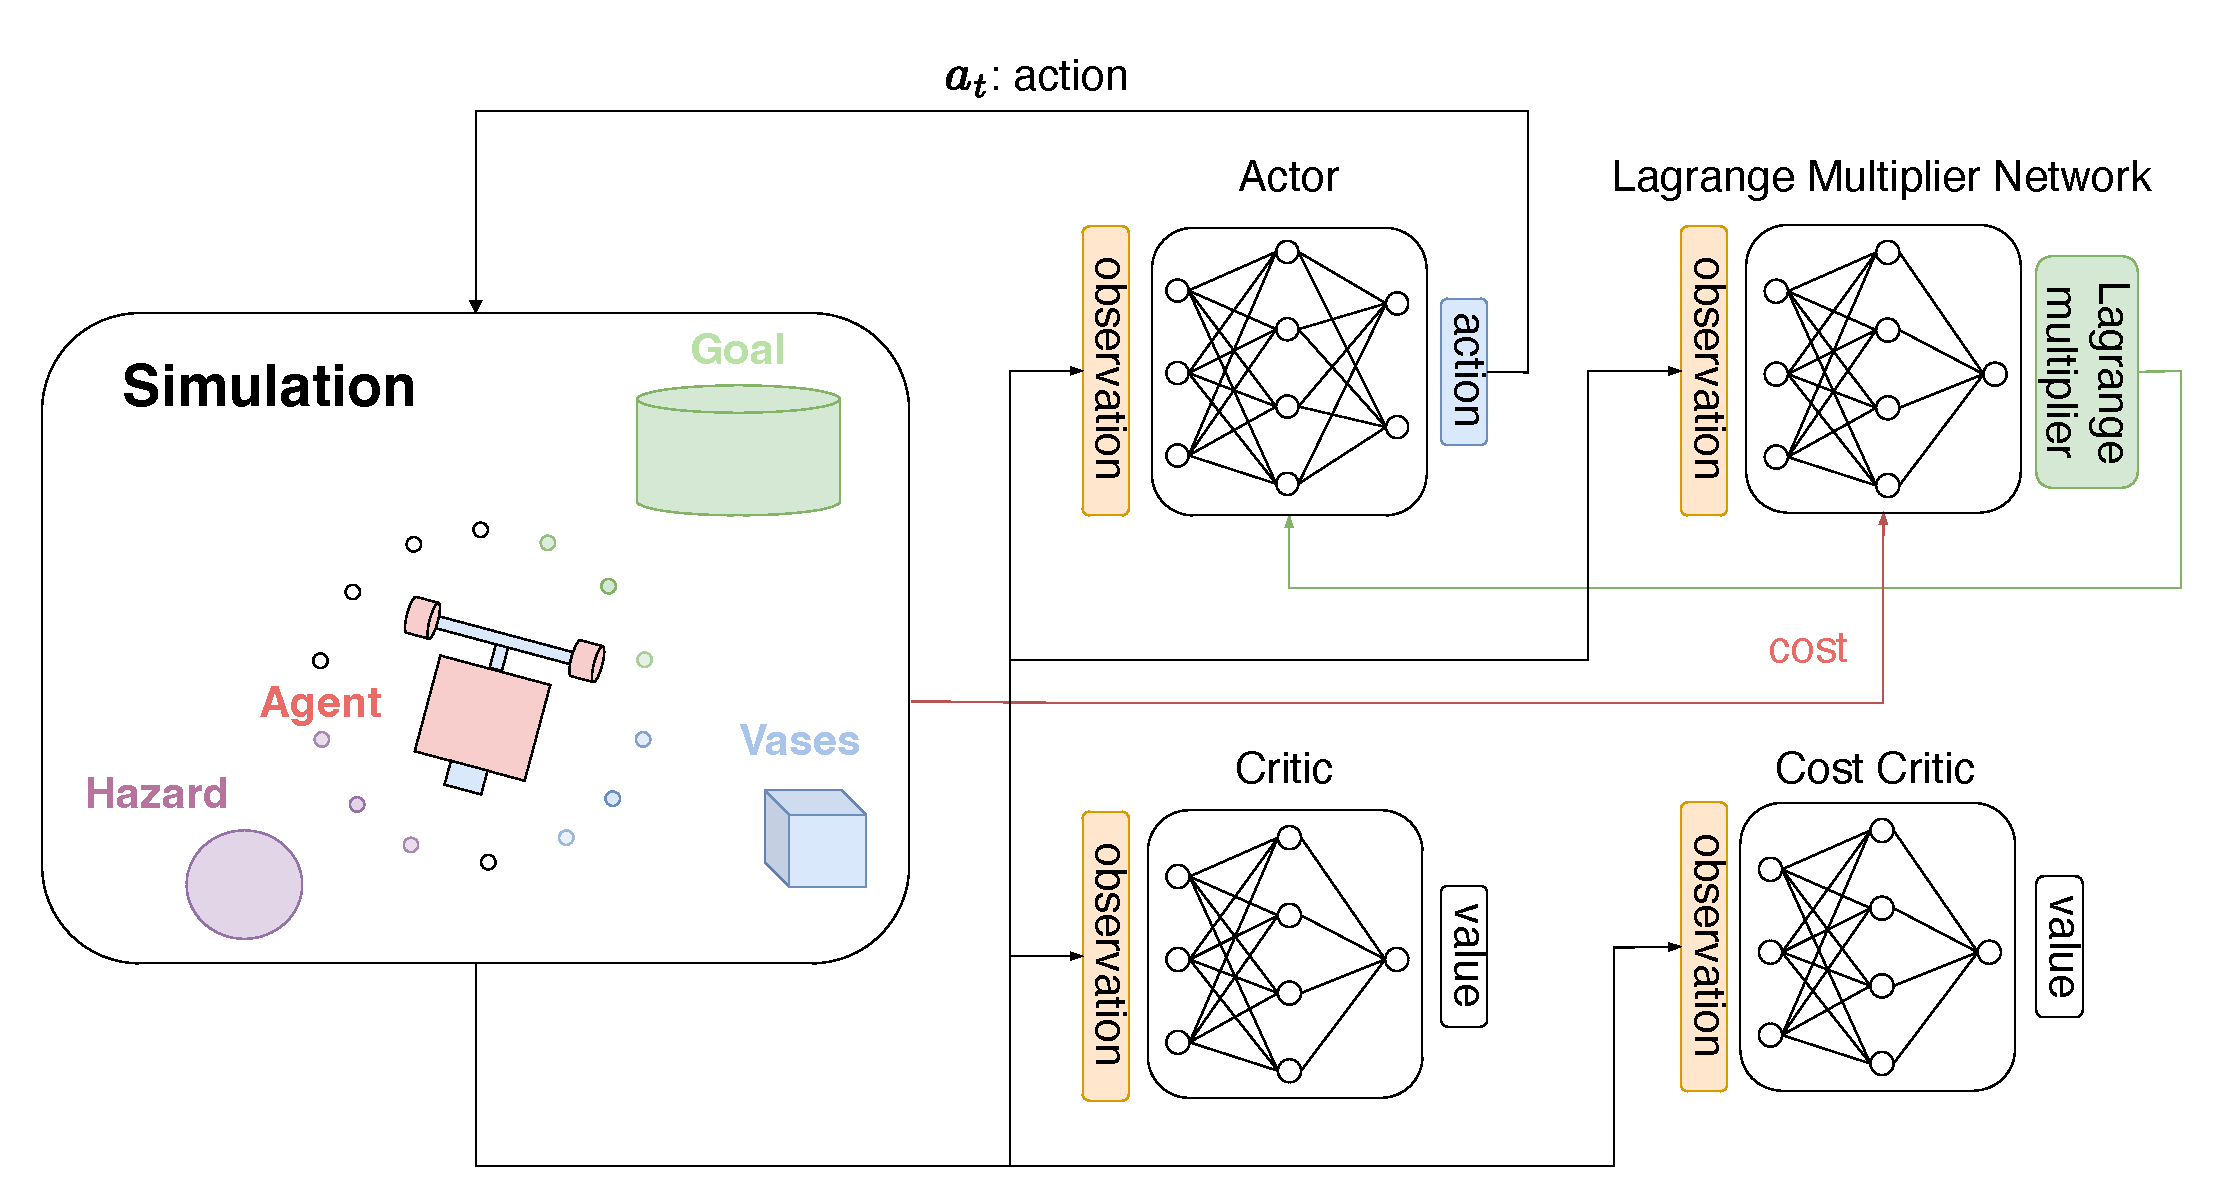
\includegraphics[width=0.6\textwidth]{figures/ppo-lagnet.pdf}
    \caption{Overview of the proposed method}
  \end{figure}

\end{frame}


\begin{frame}{\insertsubsectionhead}{Comparison of Methods}

  {
    \begin{figure}
      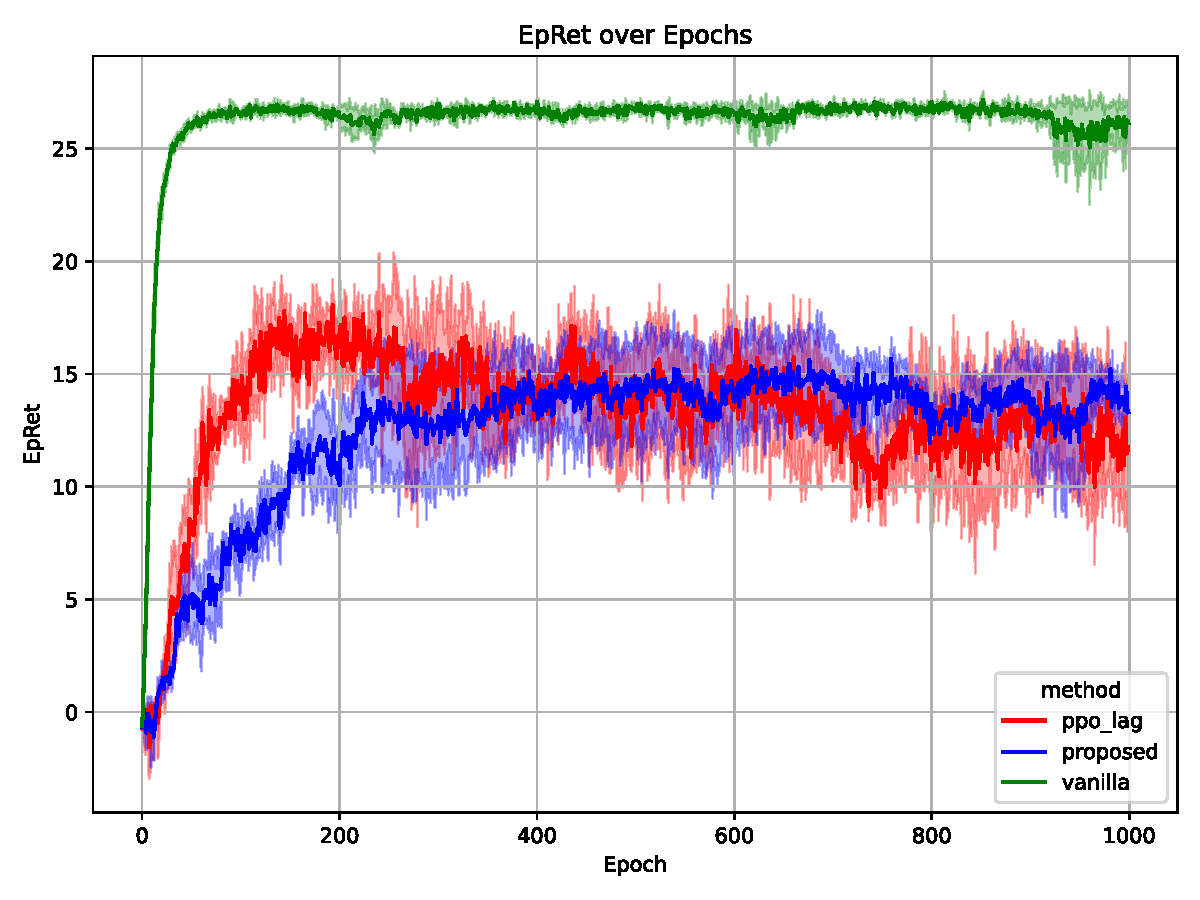
\includegraphics[width=0.45\textwidth]{figures/result_reward.pdf}
      \hspace{1cm}
      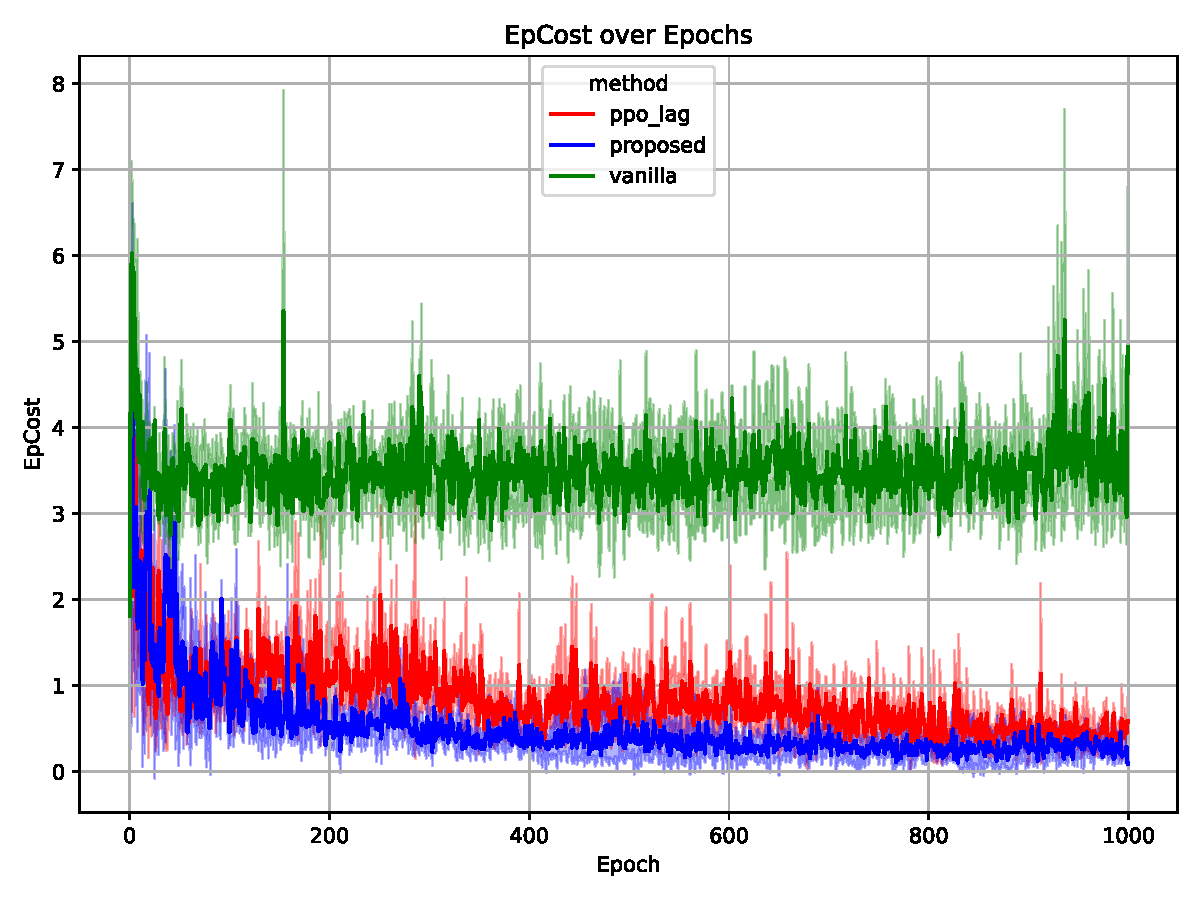
\includegraphics[width=0.45\textwidth]{figures/result_cost.pdf}
      \caption{Performance comparison on Safety Gym Point Goal tasks}
    \end{figure}
  }

\end{frame}

\note[enumerate]
{
  \item This figure shows the performance comparison on Safety Gym Point Goal tasks.
  \item The left graph shows the cumulative reward, and the right graph shows the cumulative cost.
  \item As you can see, the proposed method achieves higher rewards while maintaining lowest costs compared to other methods.
}

\begin{frame}{\insertsubsectionhead}{Comparison of Methods}

  \centering
  \begin{columns}[T,totalwidth=\textwidth]
    % PPO
    \column{0.32\textwidth}
      \centering
      \textbf{PPO}
      \includemedia[
        width=\linewidth,
        height=0.5625\linewidth,
        activate=pageopen,
        addresource=figures/ppo-5121.mp4,
        flashvars={source=figures/ppo-5121.mp4&autoPlay=true&loop=true}
      ]{}{VPlayer.swf}

    % PPO Lagrangian
    \column{0.32\textwidth}
      \centering
      \textbf{PPO Lagrangian}
      \includemedia[
        width=\linewidth,
        height=0.5625\linewidth,
        activate=pageopen,
        addresource=figures/ppo_lag-5121.mp4,
        flashvars={source=figures/ppo_lag-5121.mp4&autoPlay=true&loop=true}
      ]{}{VPlayer.swf}

    % Proposed Method
    \column{0.32\textwidth}
      \centering
      \textbf{Proposed Method}
      \includemedia[
        width=\linewidth,
        height=0.5625\linewidth,
        activate=pageopen,
        addresource=figures/ppo_lagnet-5121.mp4,
        flashvars={source=figures/ppo_lagnet-5121.mp4&autoPlay=true&loop=true}
      ]{}{VPlayer.swf}

  \end{columns}

\end{frame}

\note[enumerate]
{
  \item This is a test video.
  \item In the case of PPO, since it does not take constraints into account, we can see that the agent steps on obstacles.
  \item Even with constrained RL, because the constraint is imposed at the trajectory level, constraint violations still occur.
  \item In contrast, with the proposed method, the constraints are considered more finely, and we can see that the agent satisfies the constraint.
}

\begin{frame}{\insertsubsectionhead}{Limitations of the Proposed Method}

  Limitations of the Proposed Approach

  \begin{itemize}
    \item<1-> Sensitivity to Lagrange multiplier (init., learning rate)
    \item<2-> Constraint threshold setting is difficult
      \begin{itemize}
        \item<2-> Too strict → overly conservative policy
        \item<2-> Too lenient → constraints not enforced
      \end{itemize}
    \item<3-> Needs sufficient violations during training
  \end{itemize}

\end{frame}

\note[enumerate]
{
  \item However, the proposed method also has some limitations.
  \item First, the Lagrangian method itself is inherently sensitive to the initial value and the learning rate.
  \item Second, setting the constraint threshold is difficult.
  \item If it is set too strictly, the policy becomes overly conservative, and if it is set too loosely, the constraints are not enforced.
  \item Lastly, since enough constraint violations are required for training, therefore, training has to be conducted in a simulation environment.
}

% ============================================
%         Conclusion Page
% ============================================


\section{Conclusion}

%~~~~~~~~~~~~~~~~~~~~~~~~~~~~~~~~~~~~~~~~~~~~~~~~~~~~~~~~~~~~~~~~~~~~~~~~~~~~~~
\subsection{Summary}

\note[enumerate]
{
  \item Finally, the conclusion.
  \item I will briefly summarize what I have explained so far.
  \item And I will also explain what I plan to do in the future.
}

\begin{frame}{\insertsubsectionhead}

  \begin{itemize}
    \item <2-> Challenges in applying RL to the real world
    \item <3-> Reward engineering is needed for diverse behaviors
    \item <4-> Constrained RL enables learning without reward engineering
    \item <5-> Constrained RL imposes constraints at the trajectory level
    \item <6-> Extension to state-wise constrained RL
  \end{itemize}

  \vspace{0.5cm}

  \uncover<7->{\textbf{But there are still challenges to solve..}}

\end{frame}

\note[enumerate]
{
  \item There are several challenges in applying reinforcement learning to the real world.
  \item To make an agent learn diverse behaviors, reward engineering is required.
  \item However, constrained RL allows learning without reward engineering.
  \item In constrained RL, constraints are imposed at the trajectory level.
  \item In my master's thesis, I extended this to state-wise constrained RL.
  \item However, there are still challenges to solve.
}

%~~~~~~~~~~~~~~~~~~~~~~~~~~~~~~~~~~~~~~~~~~~~~~~~~~~~~~~~~~~~~~~~~~~~~~~~~~~~~~

\subsection{Future Work}

\begin{frame}{\insertsubsectionhead}

  \begin{itemize}
    \item <2-> Hard to set appropriate constraint threshold $\rightarrow$ Curriculum learning \cite{weng2020curriculum, kim2024not}
  \end{itemize}

  \uncover<2->{
    \begin{figure}
      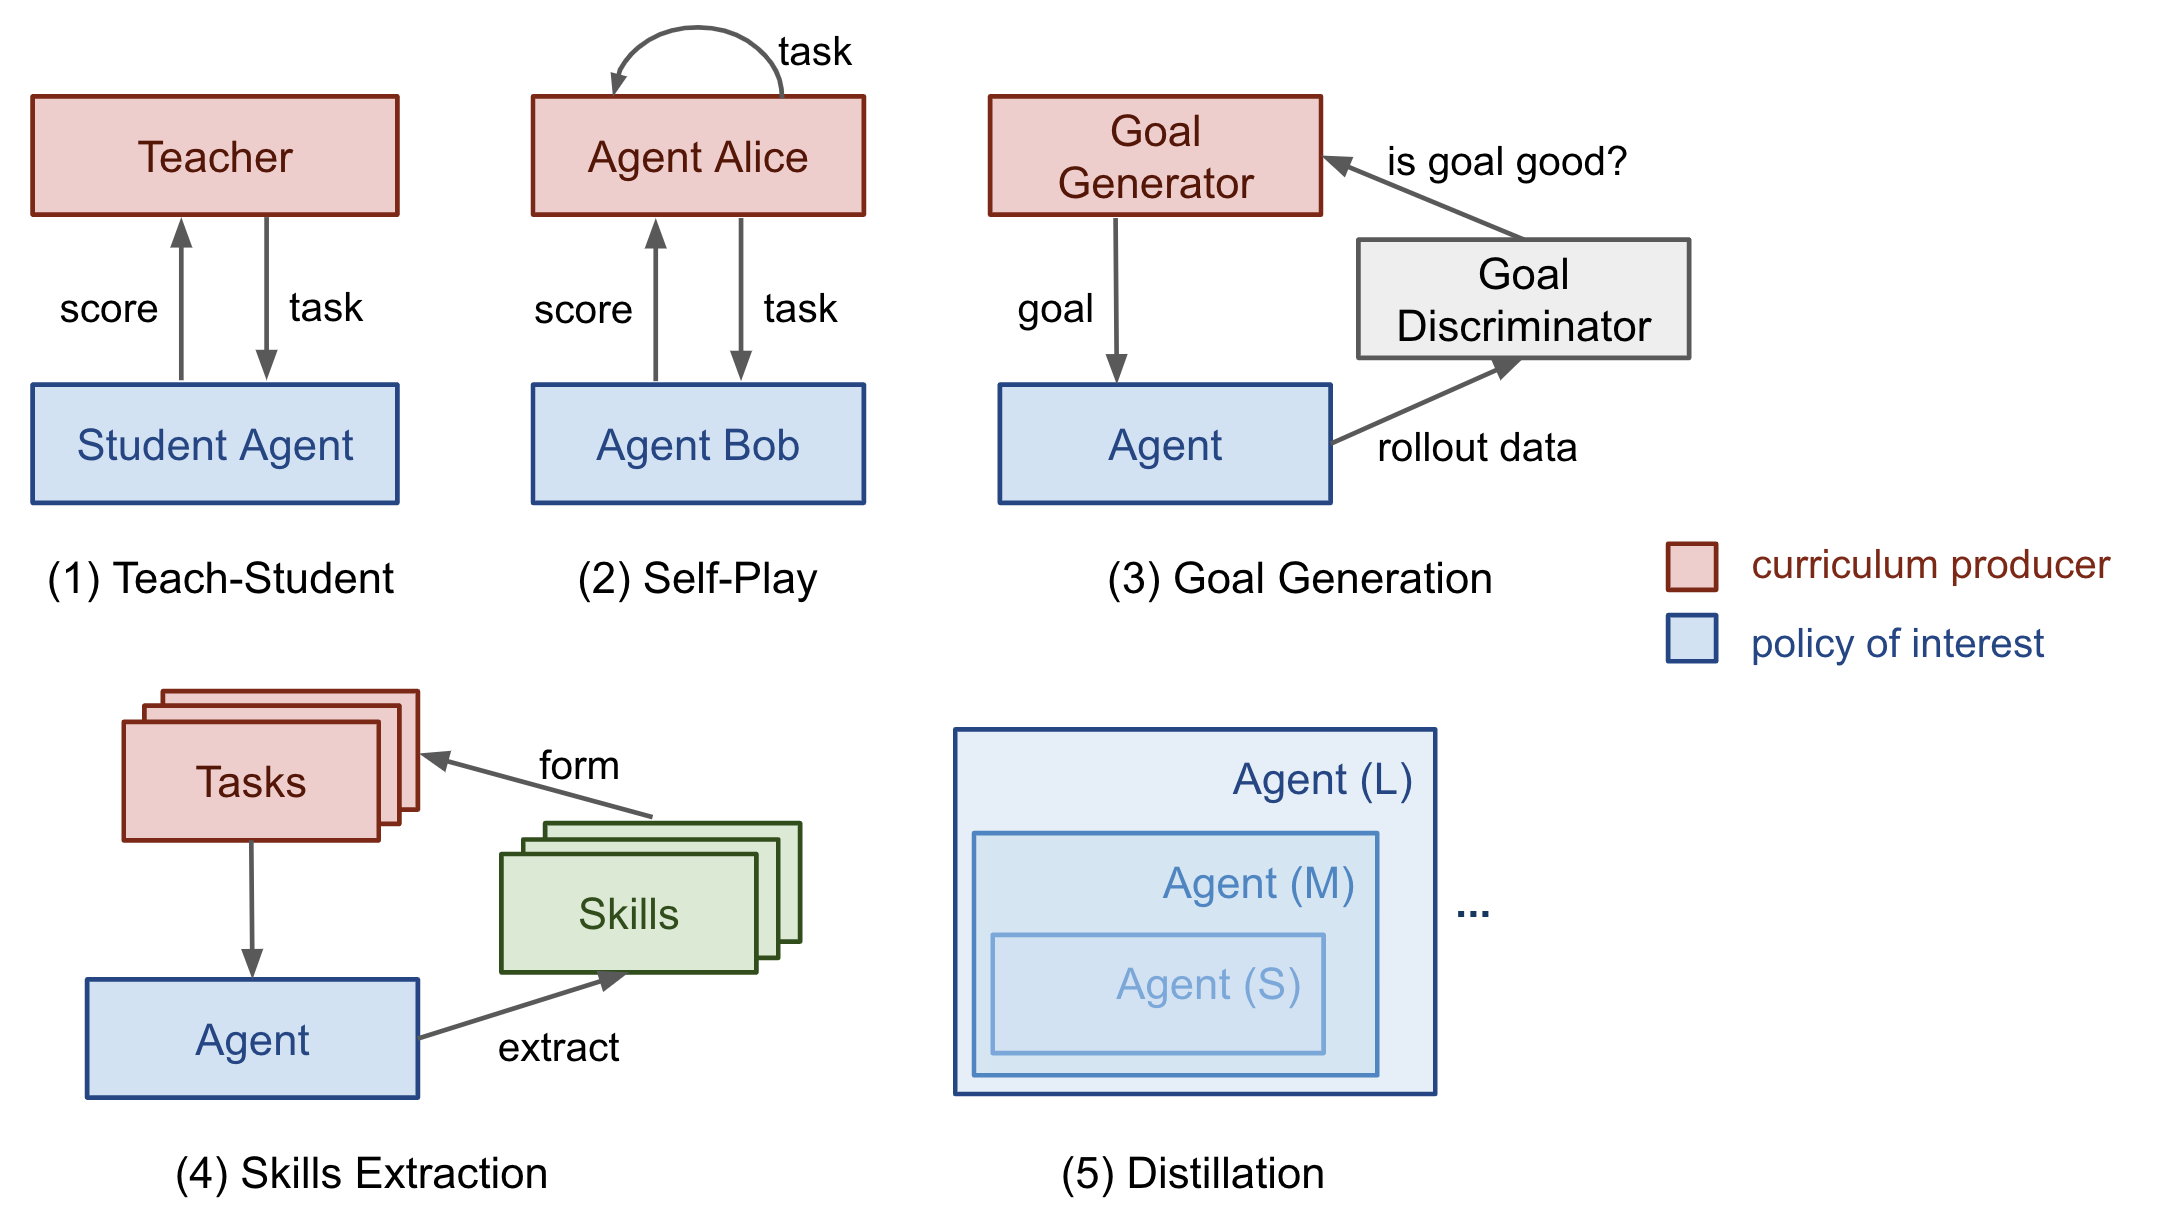
\includegraphics[width=0.3\textwidth]{figures/curriculum-learning.png}
      \caption{Curriculum learning overview}
    \end{figure}
  }

  \begin{itemize}
    \item <3-> Constraint violations during training $\rightarrow$ Combine with Model-Based methods \cite{chua2018deep, liu2020safe, jayant2022model, paolo2022guided}
  \end{itemize}

  \vspace{0.5cm}
  
  \uncover<3->{
    \begin{figure}
      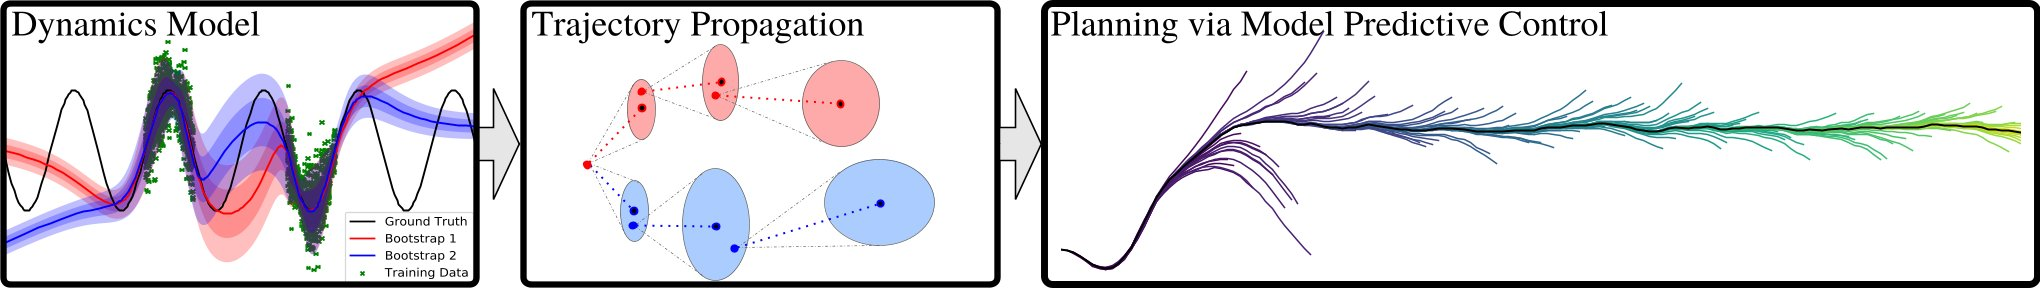
\includegraphics[width=0.4\textwidth]{figures/model-based.jpg}
      \caption{Model-Based RL overview}
    \end{figure}
  }

\end{frame}

\note[enumerate]
{
  \item First, there is the problem of setting an appropriate codenstriant threshold.
  \item To address this, I think curriculum learning can be helpful, where the agent starts with easier tasks and gradually moves to more difficult ones.
  \item This can support setting appropriate constraint thresholds.
  \item In addition, there is the issue that, during training, the agent must frequently violate the constraints.
  \item To reduce this, I expect that combining model-based methods can be helpful.
  \item By using a learned model for planning, the agent can learn safe policies with fewer constraint violations.
}

%~~~~~~~~~~~~~~~~~~~~~~~~~~~~~~~~~~~~~~~~~~~~~~~~~~~~~~~~~~~~~~~~~~~~~~~~~~~~~~

% ============================================
%         Thank you Page
% ============================================

\section{}
\begin{frame}{}
    \centering \Large
    \emph{Thank you for your attention!}
\end{frame}

\note[enumerate]
{
  \item This concludes my presentation.
  \item Thanky you for your attention.
  \item If you have any questions, please feel free to ask.
}

%~~~~~~~~~~~~~~~~~~~~~~~~~~~~~~~~~~~~~~~~~~~~~~~~~~~~~~~~~~~~~~~~~~~~~~~~~~~~~~

%~~~~~~~~~~~~~~~~~~~~~~~~~~~~~~~~~~~~~~~~~~~~~~~~~~~~~~~~~~~~~~~~~~~~~~~~~~~~~~
\begin{frame}[allowframebreaks]{References}

  \bibliography{localRefs}
  \bibliographystyle{IEEEtran}

\end{frame}
%~~~~~~~~~~~~~~~~~~~~~~~~~~~~~~~~~~~~~~~~~~~~~~~~~~~~~~~~~~~~~~~~~~~~~~~~~~~~~~

\end{document}